\documentclass{fenics}
\begin{frame}
\frametitle{Notation}
\begin{tabular}{l|l}
\bf{Symbol} & \bf{Explanation}  \\
\hline
$( \ )_F,(\ )_S,(\ )_M$ & fluid, structure, mesh \\
\uncover<2->{capital letters} & \uncover<2->{reference configuration} \\
\uncover<3->{lowercase letters} & \uncover<3->{deformed configuration} \\
\uncover<4->{$\rho$}   & \uncover<4->{density} \\
\uncover<5->{$\Sigma$} & \uncover<5->{stress tensor} \\
\uncover<6->{$D$}      & \uncover<6->{displacement} \\
\uncover<7->{$U$}      & \uncover<7->{velocity} \\
\uncover<8->{$P$}      & \uncover<8->{pressure} \\
\uncover<9->{$F$}      & \uncover<9->{deformation gradient} \\
\uncover<10->{$J$}     & \uncover<10->{Jacobian determinant} \\
\uncover<11->{$\Omega$}& \uncover<11->{domain} \\
\uncover<12->{$\GammaFS$} &\uncover<12->{fluid-structure interface} \\
\end{tabular}
\end{frame}

\fenicstitle{Automatic differentiation of a fluid-structure interaction problem}
            {Gabriel Balaban, Anders Logg, \\ Marie E. Rognes}
            {Simula Research Laboratory \\ University of Oslo}
            {FEniCS Worksop 2013, Cambridge}
            {2013--03--18}

\begin{document}
\begin{frame}

  \begin{columns}

    \begin{column}{0.75\textwidth}
      \titlepage
    \end{column}

    \begin{column}{0.25\textwidth}
      \begin{center}
        \includegraphics[width=\textwidth]{png/bloodvessel.png}
      \end{center}
    \end{column}

  \end{columns}

\end{frame}

\begin{frame}
  \frametitle{Examples of Fluid--structure interaction}

  \begin{center}
   \fbox{ 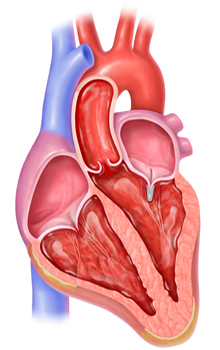
\includegraphics[height=0.4\textheight]{jpg/HeartMitralValve.jpg}}
    \hspace{0.5cm}
   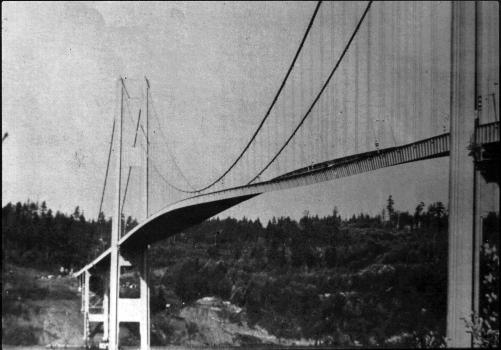
\includegraphics[height=0.4\textheight]{jpg/TacomaNarrows.jpg}
  \end{center}
  
\uncover<2->{Modelling Challenges}
  \begin{itemize}
  \item<2->model must integrate solid and fluid mechanics
   \item<3->fluid geometry depends on structure deformation
  \end{itemize}
\end{frame}

\begin{frame}
  \frametitle{Solving the FSI problem}

  Issues:
  \begin{itemize}
  \item<2->
    Continuum mechanics formulation
  \item<3->
    Partitioned vs monolithic
  \item<4->
    Fixed-pointed vs Newton
  \item<6->
    Approximation of the Jacobian
  
  \end{itemize}

  \bigskip

  \uncover<7->{In this work we:}

  \begin{itemize}
  \item<7->
    derive a \textbf{Newton's} method with exact Jacobians for FSI problems
    using the \textbf{arbitrary Lagrangian Eulerian} formulation
  \item<8->
    implement a \textbf{monolithic} solver in Python (using FEniCS)
  \item<9->
    investigate various \textbf{optimizations} and \textbf{simplifications}
  \end{itemize}

\end{frame}

\begin{frame}
  \frametitle{Setup of the FSI problem}

\begin{figure}[htbp]
  \centering
  \def\svgwidth{0.72\columnwidth}
  \input{pdf/domainsAndVariables.pdf_tex}
\end{figure}

\end{frame}

\begin{frame}
  \frametitle{Mismatch in standard fluid and solid models}

 \begin{figure}[htbp]
  \centering
  \def\svgwidth{0.72\columnwidth}
  \input{pdf/Models.pdf_tex}
\end{figure}

  
\end{frame}
\begin{frame}
  \frametitle{Mesh smoothing problem}

\begin{figure}[htbp]
  \def\svgwidth{0.6\columnwidth}
  \input{pdf/MeshProblem.pdf_tex}
\end{figure}

\uncover<2->{
Mesh equation
\begin{equation*}
\dotUM- \textrm{Div} \; \SigmaM(\UM) = 0
\end{equation*}}

\end{frame}

\begin{frame}
  \frametitle{Arbitrary Lagrangian-Eulerian framework}

\begin{figure}[htbp]
  \def\svgwidth{0.7\columnwidth}
  \input{pdf/ALE_Formulation.pdf_tex}
\end{figure}

 \uncover<2->{
 ALE time derivative:
 \begin{equation*}
  \ddt (\rho u) = \dot{\rho u} + \rho \; (\grad u \cdotp (u- \alert{\dotUM}) )
 \end{equation*}
 }

\uncover<3->{
 ALE fluid equation:
\begin{equation*}
    \begin{aligned}
         \rhoF(\dotuF + \graduF \cdot (\uF - \alert{\dotUM})) - \divsigmaFup &= \fF \quad &\textrm{in}\; \oFt \\
         \divuF &= 0 \quad  &\textrm{in} \;\oFt
       \end{aligned}
     \end{equation*}
     }
\end{frame}

\begin{frame}
  \frametitle{Interface conditions}

\begin{figure}[htbp]
  \def\svgwidth{0.3\columnwidth}
  \input{pdf/fsi_interface.pdf_tex}
\end{figure}
  
  \begin{itemize}[<+->]
 \item
  Stress continuity:
  \begin{equation*}
    \sigmaS \cdot n = \sigmaF \cdot n
    \quad \text{ on } \gammaFS
  \end{equation*}
 \item
  Kinematic continuity:
  \begin{equation*} 
    \uF = \uS
    \quad \text{ on } \gammaFS
   \end{equation*}
 \item
  Domain continuity:
  \begin{equation*}
    \dM = \dStruc
    \quad \text{ on } \gammaFS
  \end{equation*}
\end{itemize}
\end{frame}

\begin{frame}
  \frametitle{Linearization of the FSI problem}
  
  Two challenges:
  \begin{itemize}
  \item<2->
    Derivative of fluid equation with respect to geometry?
      \begin{equation*}
      \begin{array}{rlll}
        \ddt (\rho u) - \divsigmaFup & = & \fF &\quad \textrm{in}\;
       \alert{\oFt}\\
        \divuF & =& 0 &\quad  \textrm{in}\; \alert{\oFt}
      \end{array}
    \end{equation*}
  \item<3->
  Linearization of essential BCs
  \begin{equation*} 
    \uF = \uS
    \quad \text{ on } \alert{\gammaFS}
   \end{equation*}
  \begin{equation*}
    \dM = \dStruc
    \quad \text{ on } \alert{\gammaFS}
  \end{equation*}
  \end{itemize}
\end{frame}

\begin{frame}
  \frametitle{The reference domain approach}

  \begin{figure}[htbp]
  \centering
  \def\svgwidth{0.3\columnwidth}
  \input{pdf/map_fluid.pdf_tex}
\end{figure}
  
  \begin{itemize}
  \item<1->
    Map the fluid problem to the reference domain
  \item<2->
    Use standard techniques to differentiate
  \item<3->
    Straightforward but tedious
  \item<4->
    \emph{Can be automated!}
  \end{itemize}
\end{frame}
 
\begin{frame}
  \frametitle{Navier--Stokes pulled back to reference domain}

  \begin{itemize}
  \item
    Equation:
    \small
    \begin{equation*}
      \begin{split}
        \rhoF\JM(\dotUF + \GradUF\cdot \FM^{-1}\cdot (\UF-\dotUM ))
        - \Divv \; \SigmaF
        & = B_{_{F}} \\
        \Divv(\JM\;\FM^{-1}\cdot\UF) & = 0
      \end{split}
    \end{equation*}
    \normalsize
  \item<2->
    Pulled-back fluid stress:
    \begin{equation*}
      \SigmaF = \JM \left(\muF(\GradUF \cdot \FM^{-1} + \FM^{-\top}\cdot 
      \GradUF ^{\top})  - \PF I \right) \cdot\FM^{-\top}
    \end{equation*}
  \end{itemize}

\end{frame}

\begin{frame} 
  \frametitle{Interface conditions: How to linearize?}
\begin{figure}[htbp]
  \def\svgwidth{0.3\columnwidth}
  \input{pdf/fsi_interface.pdf_tex}
\end{figure}
  
  Stress continuity:
  \begin{equation*} \label{eq:continuity,stress}
    \SigmaS \cdot N = \SigmaF \cdot N
    \quad \text{ on } \GammaFS
  \end{equation*}

  Kinematic continuity:
  \begin{equation*} \label{eq:continuity, kinematic}
    \UF = \PS
    \quad \text{ on } \GammaFS
  \end{equation*}

  Domain continuity:
  \begin{equation*} \label{eq:continuity, domain}
    \DM = \DS
    \quad \text{ on } \GammaFS
  \end{equation*}
\end{frame}

\begin{frame}
  \frametitle{Linearization of essential boundary conditions}

  Introduce Lagrange multipliers $(\tauF, \tauM)$ and corresponding
  trial functions $(\chiF, \chiM)$

  \bigskip

  Kinematic continuity:
  \begin{displaymath}
     \inner{\UF - \PS}{\tauF}_{\GammaFS} + \inner{\chiF}{\vF}_{\GammaFS}
  \end{displaymath}

  Domain continuity:
  \begin{displaymath}
     \inner{\DM - \DS}{\tauM}_{\GammaFS} + \inner{\chiM}{\vM}_{\GammaFS}
  \end{displaymath}

\end{frame}

\begin{frame}
  \frametitle{The linearized FSI operator (the Jacobian)}

  \begin{columns}

    \begin{column}{0.5\textwidth}
      \includegraphics[width=\textwidth]{png/jacobian.png}
    \end{column}

    \begin{column}{0.5\textwidth}
      \includegraphics[width=\textwidth]{pdf/jacobian.pdf}
    \end{column}

  \end{columns}

\end{frame}

\begin{frame}[fragile]
  \frametitle{FEniCS implementation}

  \vspace{0.5cm}

  \begin{center}
    \tt J = derivative(R, U)
  \end{center}

\end{frame}
 
\begin{frame}
  \frametitle{An analytic test problem}

  \vspace{1cm}
  \def\svgwidth{1.1\textwidth}
  \import{pdf/}{pdf/analyticproblem.pdf_tex}
  
  Primary variables:
  \begin{displaymath}
    \begin{split}
       \UF &= y(1 - y)\sin{t} \\
       \PF &= 2C\sin{t}(1 - x -Cxy(1 -y)(1 -\cos{t})) \\
       \DS &= Cy(1 - y)(1 - \cos{t})  \\
       \PS &= Cy(1 - y)\sin{t} \\
       \DM &= Cxy(1 -y)(1 -\cos{t}) \\
    \end{split}
  \end{displaymath}
%   
%   \begin{itemize}
%   \item
%     Test Newton's method (quadratic convergence)
%   \item
%     Test finite element formulation (convergence in $h$ and $\mathrm{d}t$)
%   \end{itemize}

\end{frame}

\begin{frame}
  \frametitle{Convergence for analytic test problem}

  \begin{center}
    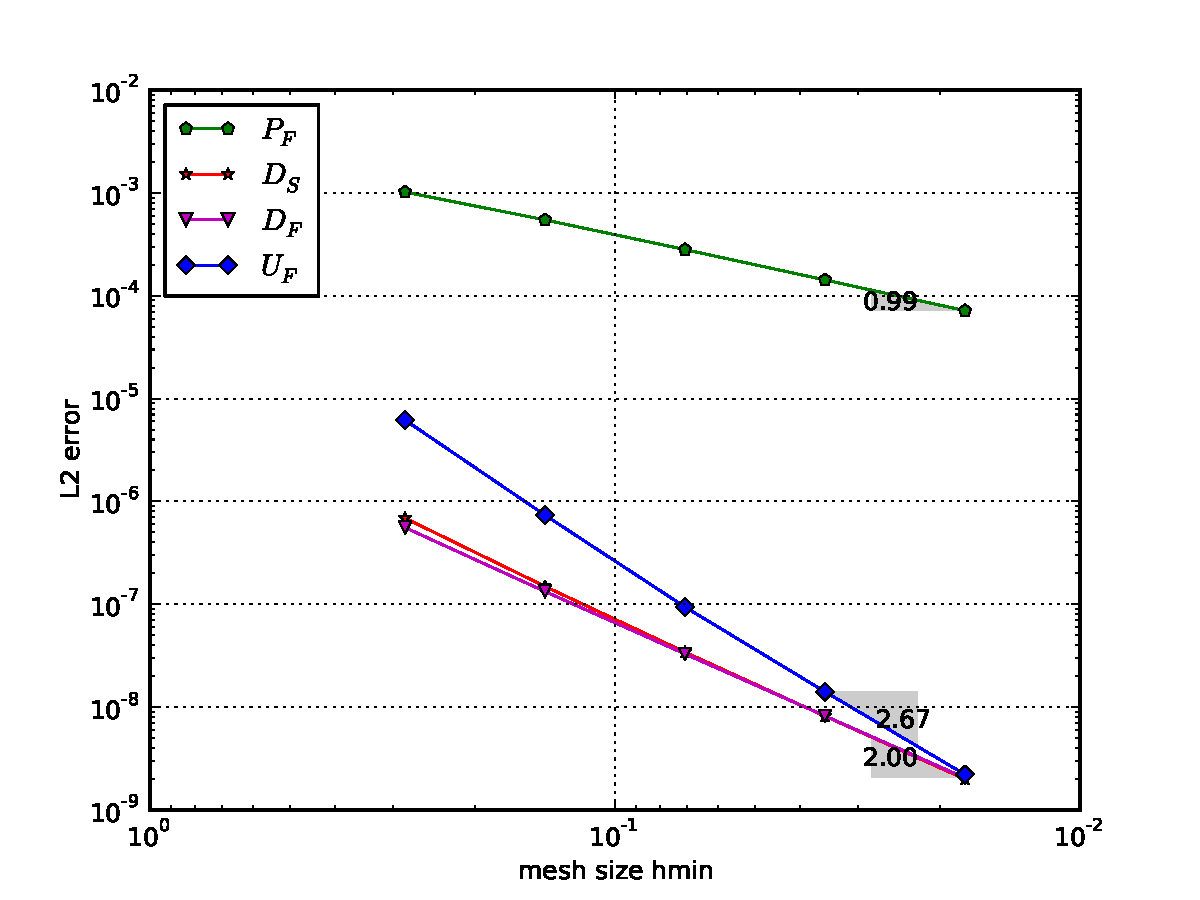
\includegraphics[width=\textwidth]{pdf/convergence1k.pdf}
  \end{center}

\end{frame}

\begin{frame}
  \frametitle{A two-dimensional blood vessel}

  \begin{center}
    \includegraphics[width=0.35\textwidth,angle=90]{png/bloodvessel0.png}
    \includegraphics[width=0.35\textwidth,angle=90]{png/bloodvessel10.png}
    \includegraphics[width=0.35\textwidth,angle=90]{png/bloodvessel20.png}
    \includegraphics[width=0.35\textwidth,angle=90]{png/bloodvessel30.png} \\
    \includegraphics[width=0.35\textwidth,angle=90]{png/bloodvessel40.png}
    \includegraphics[width=0.35\textwidth,angle=90]{png/bloodvessel50.png}
    \includegraphics[width=0.35\textwidth,angle=90]{png/bloodvessel60.png}
    \includegraphics[width=0.35\textwidth,angle=90]{png/bloodvessel140.png}
  \end{center}

\end{frame}

\begin{frame}
  \frametitle{Break-down of run-time}

  \small
  \begin{tabular}{|l|l|r|r|r|}
    \hline
    \bf{Problem} & \bf{Routine} & \bf{Calls} & \bf{Time} (s) & \\
    \hline
    \bf{Analytic problem} &Jacobian assembly&   28 & 83.9s & \textbf{90\%} \\
    mesh size = 231        &Linear solve&        28 & 1.86s & 2\% \\
    time steps = 10       &Residual assembly&   38 & 0.915s  & 1\% \\
    &&&&\\
    \hline
    \bf{Blood vessel} &Jacobian assembly&   343 & 2980s & \textbf{81\%} \\
    mesh size = 1271    &Linear solve&        343 & 254s & 18\% \\
    time steps = 140    &Residual assembly&   483 & 64.1s &  1\%  \\
    &&&&\\
    \hline
  \end{tabular}
  \normalsize

\end{frame}

\begin{frame}
  \frametitle{Effect of Jacobian reuse}

  \small
  \begin{tabular}{|l|l|l|l|}
    \hline
    \bf{Problem} & \bf{Routine} & \bf{Calls}  & \\
    \hline
    \bf{Analytic problem} &Jacobian assembly&     1 (-27)               & -95 \% \\
    mesh size = 231        &Linear solve&        51 ({\color{red}+23})  & -96\% \\
    time steps = 10        &Residual assembly&   61 ({\color{red}+23})  & {\color{red}+54\%} \\
                           &\bf{Total Runtime:} &                       & \bf{-93} \% \\

    &&&\\
    \hline
    \bf{Blood vessel}&Jacobian assembly&   25 (-308) & -93 \% \\
    mesh size = 1271    &Linear solve&        1287 ({\color{red}+944}) & -92 \% \\
    time steps = 140    &Residual assembly&   1427 ({\color{red}+944}) & {\color{red}+192}\%  \\
                        &\bf{Total}       &                            & \bf{-91 \%} \\
    \hline
  \end{tabular}
  \normalsize

\end{frame}

\begin{frame}
  \frametitle{Effect of Jacobian reuse}

  \begin{center}
    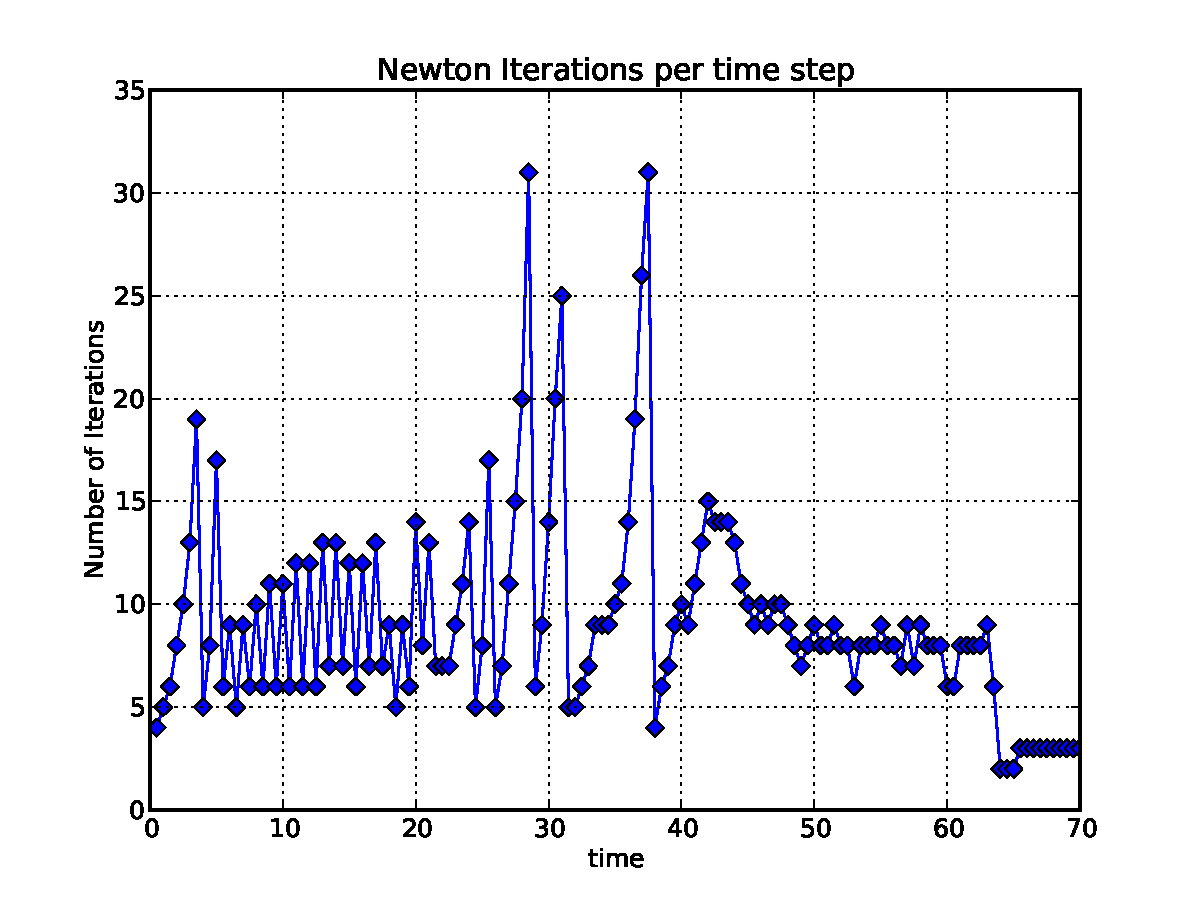
\includegraphics[width=\textwidth]{pdf/newtoniter.pdf}
  \end{center}

\end{frame}

\begin{frame}
  \frametitle{Optimization summary}

  \begin{center}
    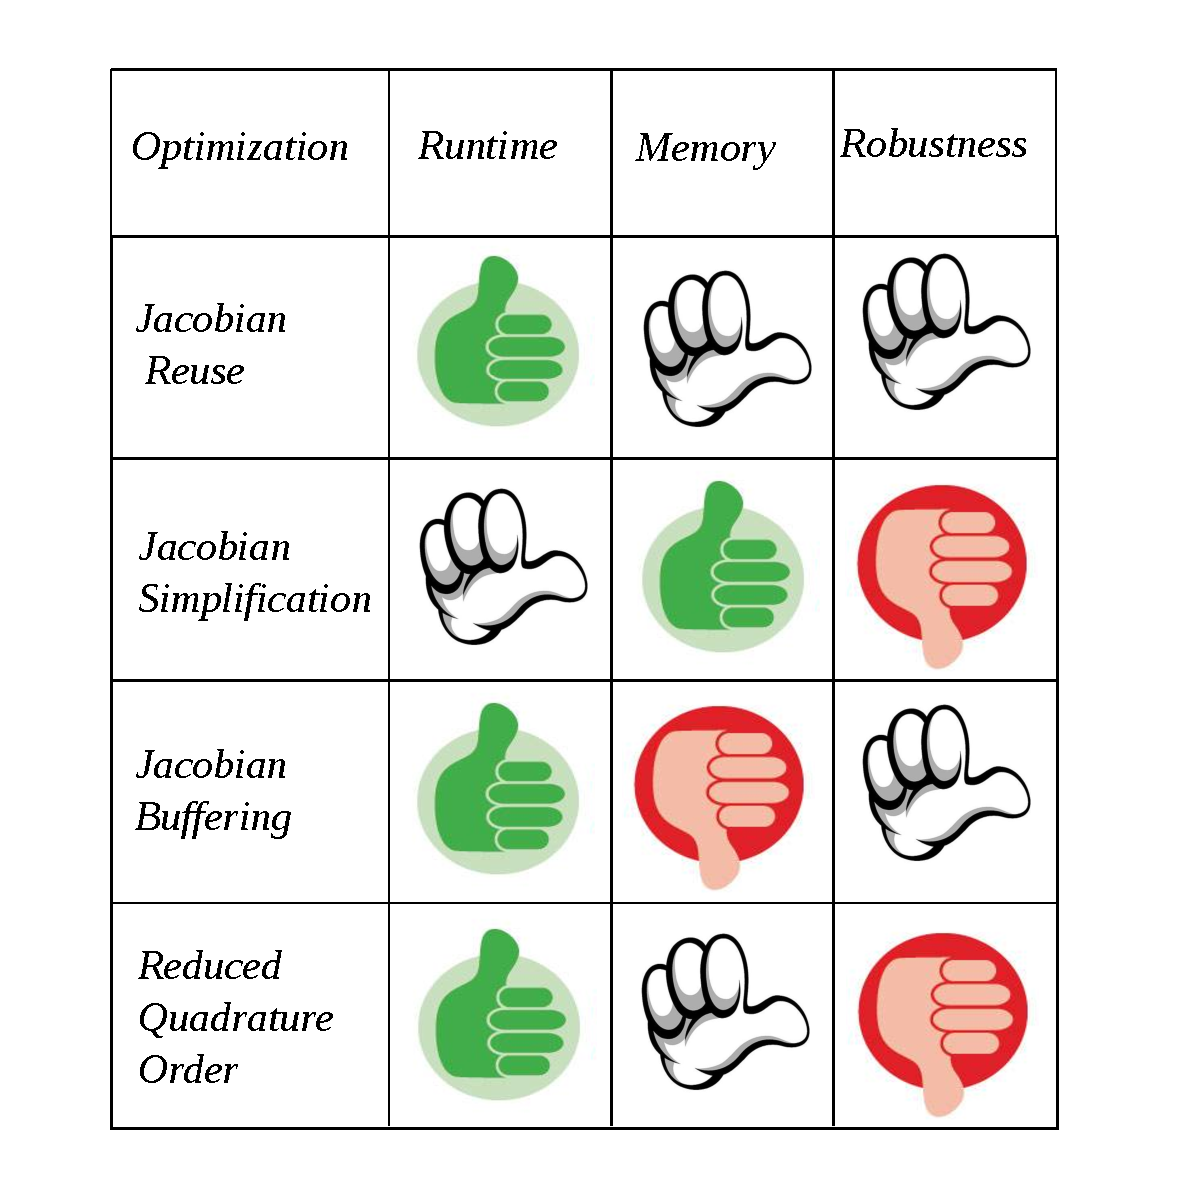
\includegraphics[width=0.7\textwidth]{pdf/optimizationsummary.pdf}
  \end{center}

\end{frame}

\begin{frame}
  \frametitle{Summary: How to use the automatic derivative to solve FSI problems}

 \begin{columns}
  \begin{column}{0.6\textwidth}
  \begin{itemize}
  \item
    Map the fluid equation to the reference domain
  \item<2->
    Impose essential BC's using Lagrange multipliers
  \item<3->
    Let the automatic derivative compute the Jacobian 
  \end{itemize}
\end{column}
    \begin{column}{0.4\textwidth}
     \includegraphics[width=\textwidth,angle=90]{png/bloodvessel40.png}
    \end{column}  
  \vspace{1cm}
\end{columns}

\uncover<4->{Challenges / work in progress:}
  \begin{itemize}
  \item<4->
    Long FFC compilation times
  \item<5->
    Preconditioning
  \end{itemize}

\end{frame}

%Get from Gabriel: Newton vs fixed-point
%Get from Gabriel: timings for compiling
%Get from Gabriel: new plot with LaTeX for fig 13 and slopes
%Marie: name of x
 %%Redo conclusions page to show picture and one or two points open to discussion.
 %%Maybe include future work? Clean up the implementation.
\end{document}